%%%%%%%%%%%%%%%%%%%%%%%%%%%%%%%%%%%%%%%%%%%%%%%%%%%%%%%%%%%%%%%%%%%%%%%%%%%%%%%%%%%%%%%%%%%%%%%%%%%
%%%%%%%%%%%%%%%%%%%%%%%%%%%%%%%%%%%%%%%%%%%%%%%%%%%%%%%%%%%%%%%%%%%%%%%%%%%%%%%%%%%%%%%%%%%%%%%%%%%
%%%%%%%%%%%%%%%%%%%%%%%%%%%%%%%%%%%%%%%%%%%%%%%%%%%%%%%%%%%%%%%%%%%%%%%%%%%%%%%%%%%%%%%%%%%%%%%%%%%
%%%%%%%%%%%%%%%%%%%%%%%%%%%%%%%%%%%%%%%%%%%%%%%%%%%%%%%%%%%%%%%%%%%%%%%%%%%%%%%%%%%%%%%%%%%%%%%%%%%

\chapter{Variables aleatorias}

%%%%%%%%%%%%%%%%%%%%%%%%%%%%%%%%%%%%%%%%%%%%%%%%%%%%%%%%%%%%%%%%%%%%%%%%%%%%%%%%%%%%%%%%%%%%%%%%%%%
%%%%%%%%%%%%%%%%%%%%%%%%%%%%%%%%%%%%%%%%%%%%%%%%%%%%%%%%%%%%%%%%%%%%%%%%%%%%%%%%%%%%%%%%%%%%%%%%%%%

\section{Medidas}

Un primer motivo para esta sección es enfatizar que, formalmente, una variable aleatoria se concibe 
como un espacio de medida y no como un recuento de eventos. 
Paralelamente, introducir la terminología adecuada permitirá entender los teoremas que dan base
a los análisis realizados.

\begin{definicion}[$\boldsymbol{\sigma}$-álgebra]
Sea $U$ un conjunto y $\mathcal{U}$ una colección de subconjuntos de $U$. Se dice que $\mathcal{U}$
es una $\sigma$-álgebra si cumple que
\begin{itemize}
\item $U \in \mathcal{U}$
\item $A \in \mathcal{U}$ implica que $A^{C} \in \mathcal{U}$
\item Si $\{ A_n \}_{n\in \mathbb{N}}$ son conjuntos tales que $A_i \in \mathcal{U}$, entonces
$\displaystyle \cup_{n\in \mathbb{N}} A_n \in \mathcal{U}$
\end{itemize}
Donde $A^{C}$ es el complemento $\{ u \in U | u \notin A \} $
\end{definicion}

Por simplicidad, en este trabajo sólo se usarán medidas para conjuntos de números reales derivadas 
de la $\sigma$-álgebra de Borel, que es definida como la $\sigma$-álgebra más pequeña que contiene a 
los intervalos abiertos abiertos\footnote{Si una $\sigma$-álgebra contiene a todos los
intervalos abiertos, entonces debe contener a todos los elementos de la $\sigma$-álgebra de Borel}.

\begin{definicion}[Medida]
Sea $U$ un conjunto y $\mathcal{U}$ una $\sigma$-álgebra definida en $U$. Se dice que una función
$\mu : \mathcal{U} \rightarrow \R \cup {\infty}$ es una medida si cumple que
\begin{itemize}
\item $\mu(\emptyset) = 0$
\item $\mu(A) \geq 0$ para cualquier $A \in \mathcal{U}$
\item Si $\{ A_n \}_{n\in \mathbb{N}}$ son conjuntos disjuntos a pares y tales que 
$A_i \in \mathcal{U}$, entonces 
$\displaystyle \mu\left( \cup_{n\in \mathbb{N}} A_n \right) = \sum_{n\in \mathbb{N}} \mu(A_n)$
\end{itemize}
Donde $\emptyset$ es el conjunto vacío %y $\R^{*} = \R \cup \{-\infty,\infty \}$
\end{definicion}

\begin{definicion}[Medida de probabilidad en $\boldsymbol{\R}$]
Sea $\mathcal{B}$ la sigma álgebra de Borel definida para $\R$, se dice que una función
$P : \mathcal{B} \rightarrow [0.1]$ es una \textbf{medida de probabilidad} si cumple que
\begin{itemize}
\item $P(\emptyset) = 0$
\item $0 \leq P(A) \leq 1$ para cualquier $A \in \mathcal{B}$
\item Si $A, B \in \mathcal{B}$ y $A\cap B = \emptyset$, entonces $P(A \cup B) = P(A) + P(B)$ 
\item $P(\R) = 1$
\end{itemize}
\label{variable_aleatoria}
\end{definicion}

%Cabe mencionar que cuando se usa una variable aleatoria para modelar un fenómeno, existe un paso
%intermedio en que los eventos relevantes se asocian con números reales

Otra forma de entender una variables aleatoria es a partir de su función de probabilidad
acumulada (FPA), ya que hay una correspondencia unívoca entre cada variable aleatoria y su FPA.

\begin{definicion}[Función de Probabilidad Acumulada]
Sea 
\begin{equation*}
F_X (x) = P\left( (-\infty,x] \right)
\end{equation*}
\end{definicion}

Habitualmente, como se hace el presente texto, se usa el símbolo $X$ para denotar a una variable 
aleatoria cuya FPA es $F_X$; bajo esta idea, para cualquier conjunto $I \subseteq \R$ se denota
$P(X \in I) = P(I)$



\begin{teorema}[Descomposición de Lebesgue]
Sea $f:I\rightarrow \R$ una función de variación acotada, con $I$ un intervalo. Entonces pueden 
hallarse funciones $f_j, f_c, f_a :I\rightarrow \R$ tales que
\begin{itemize}
\item $f = f_j+ f_c+ f_a$
\item $f_j = \sum_{y \leq x} f(x-0) + f(x+0)$
\item $f_a$ es absolutamente continua\footnote{Para que una función sea absolutamente continua,
basta que sea de variación acotada y que mapee conjuntos de medida cero en conjuntos de medida
cero} en $I$
\item $f_c$ es una función singular\footnote{Una función es singular si es continua, de 
variación acotada y no-constante, y se cumple que tiene derivada cero casi en todas partes} en 
$I$
\end{itemize}
Estas funciones son únicas excepto por constantes, y en conjunto son llamados la 
\textit{descomposición de Lebesgue} de $f$
\label{Lebesgue_decomp}
\end{teorema}

%%%%%%%%%%%%%%%%%%%%%%%%%%%%%%%%%%%%%%%%%%%%%%%%%%%%%%%%%%%%%%%%%%%%%%%%%%%%%%%%%%%%%%%%%%%%%%%%%%%

\section{Procesos estocásticos}

\begin{definicion}[Proceso estocástico]
Un proceso estocástico \xt es una familia de variables aleatorias reales, 
indexadas por $t \in T$.
\label{proc_estocastico}
\end{definicion}

Respecto al conjunto $T$ que indexa a un proceso estocástico, y que será referido como 
\textit{tiempo}, conviene introducir dos grandes grupos para los mismos
\begin{itemize}
\item \textit{Continuo} si $T$ es un intervalo cerrado
\item \textit{Discreto} si $T$ es de la forma 
$\{ t_0 + n \delta \lvert n \in U \subseteq \mathbb{Z} \}$
\end{itemize}

Los procesos a tiempo discreto contemplan conjuntos finitos e infinitos de puntos en el tiempo.
No se manejan discutirá sobre otros tipos de tiempo en este trabajo.

Como notación, se usará \xt  para el proceso estocástico y $X(t)$ para una de las variables
aleatorias que lo componen; de la misma manera $x(t)$ es una realización de $X(t)$ y $F_{X(t)}$ 
es la función de probabilidad acumulada para $X(t)$.



\begin{definicion}[Continuidad estocástica en media cuadrática]
Un proceso estocástico a tiempo continuo $\{ X(t) \}$ es estocásticamente continuo, en el 
sentido de media cuadrática, en un tiempo admisible $t_0$ si y sólo si
\begin{equation*}
\lim_{t \rightarrow t_0} \E{\left( X(t) - X(t_0) \right)^{2}} = 0
\end{equation*}
\label{cont_est}
\end{definicion}

Una forma natural de pensar en la definición \ref{cont_est} es que, si $\abso{t-t_0}$ es muy 
pequeño, entonces $X(t)$ y $X(t_0)$ difieren muy poco entre s\'i (como variables aleatorias).
Es destacable que si un proceso es estocásticamente continuo en un intervalo, sus realizaciones 
solamente se pueden garantizar continuas casi en todas partes \footnote{Una propiedad se cumple 
\textbf{casi en todas partes} si se cumple en un conjunto cuyo complemento tiene medida cero} en 
ese intervalo.

Como ejemplos, un proceso ruido blanco (definición \ref{r_blanco}) no es estocásticamente 
continuo, mientras que un proceso de Wiener (definición \ref{r_wiener}) s\'i lo es.

\begin{definicion}[Proceso ruido blanco]
Se dice de un proceso estocástico $\{ R(t) \}$ que cumple, para cualesquiera tiempos admisibles
$t$ y $s$, las siguientes propiedades:
\begin{itemize}
\item $\E{R(t)}=0$
\item $\Cov{R(t),R(s)}=0 \Leftrightarrow t=s$ 
\end{itemize}
\label{r_blanco}
\end{definicion}

\begin{definicion}[Proceso de Wiener]
Se dice de un proceso estocástico $\{ W(t) \}$ que cumple, para cualesquiera tiempos admisibles
$t$ y $s$ (con $s>t$) las siguientes propiedades:
\begin{itemize}
\item $W(0) = 0$ ($W(0)$ es constante)
\item $W(s)-W(t)$ es independiente de $W(u)$, para todo $u<t$ admisible
\item $W(s)-W(t) \sim N(0,\abso{t-s})$  (los incrementos tienen distribución normal)
\end{itemize}
\label{r_wiener}
\end{definicion}

\begin{definicion}[Estacionariedad débil]
Un proceso estocástico \xt es débilmente estacionario si y sólo si para cualesquiera tiempos 
admisibles\footnote{El término \textit{tiempos admisibles} significa que la definición es la misma
para diferentes tipos de tiempo, bajo las restricciones pertinente} $t$, $s$ se tiene que
\begin{itemize}
\item $\E{X(t)} = \mu_X$
\item $\Var{X(t)} = \sigma^{2}_X$
\item $\Cov{X(t),X(s)} = \rho_X (s-t)$
\end{itemize}
Donde $\mu_X$, $\sigma^{2}_X$ son constantes, $\rho_X(\tau)$ es una función que únicamente 
depende de $\tau$
\label{est_orden_primera}
\end{definicion}

\begin{definicion}[Función de espectro integrado]
Sea \xt un proceso a tiempo continuo, débilmente estacionario. Se define su
función de espectro integrado como
%\begin{align*}
%H(\omega_2) - H(\omega_1) &= \frac{1}{2 \pi} \int_{\omega_1}^{\omega_2} h(\lambda) d\lambda \\
%&= \frac{1}{2 \pi} \intR \frac{e^{- i \omega_2 t}-e^{- i \omega_1 t}}{- t \tau} R(\tau) d\tau
%\end{align*}
\begin{equation*}
H(\omega_2) - H(\omega_1) = 
\frac{1}{2 \pi} \intR \frac{e^{- i \omega_2 t}-e^{- i \omega_1 t}}{- i \tau} R(\tau) d\tau
\end{equation*}
Donde $h$ es la FDE para \xt
\end{definicion}

\section{Periodograma}

Una observación interesante sobre estos teoremas es el caso $\tau = 0$
\begin{equation*}
\rho(0) = \int_{-A}^{+A} dF(\omega) = F(A) - F(-A)
\end{equation*}
donde $A$ vale $\infty$ o $\pi$ según sea el caso discreto o continuo. Si $R$ es la función de
autocovarianza del proceso, entonces la ecuación anterior se traduce en que
\begin{equation*}
R(0) = \sigma^{2} \left( F(A) - F(-A) \right) = \sigma^{2} F(A)
\end{equation*}
donde $\sigma^{2}$ es la varianza del proceso. 
Esta observación adquiere importancia porque la FDE integrada ($H$), por definición, satisface 
el papel de $F$ salvo por la condición $F(\infty)=1$; si se puede garantizar que 
$H(\infty)<\infty$ entonces puede ser normalizada para satisfacer tal condición y, más aún,
si tal fuera el caso entonces $H(\infty)=\sigma^{2}$. Una consecuencia muy fuerte de este 
comentario es que, como se ha establecido previamente que sólo se considerarán procesos con
segundos momentos finitos, entonces la FDE de los procesos considerados siempre es acotada.


Se puede demostrar que $\aste{R}$ tiene las siguientes propiedades:
\begin{itemize}
\item $\E{\aste{R}(\tau)} = \left(1 - \frac{\abso{\tau}}{N} \right) R(\omega)$
\item $\Var{\aste{R}(\tau)} \approx \frac{1}{N} 
\sum_{r=-\infty}^{\infty} \left( R^{2}(r) + R(r-\tau)R(r+\tau) \right)$
\item $\Cov{\aste{\rho}(\tau),\aste{\rho}(\tau+\nu)} \approx \frac{1}{N} 
\sum_{r=-\infty}^{\infty} \left( \rho(r)\rho(r+\nu) + \rho(r-\tau)\rho(r+\tau+\nu) \right)$
\end{itemize}
Las aproximaciones para la varianza y covarianza se vuelven exactas si el proceso sigue una 
distribución normal en todos los tiempos.

%%%%%%%%%%%%%%%%%%%%%%%%%%%%%%%%%%%%%%%%%%%%%%%%%%%%%%%%%%%%%%%%%%%%%%%%%%%%%%%%%%%%%%%%%%%%%%%%%%%

\subsection{Representación espectral}

\begin{teorema}
Sea $\{X(t)\}$ un proceso estocástico a tiempo continuo débilmente estacionario de media 0 y 
estocásticamente continuo en el sentido de media cuadrática. Entonces, existe un proceso 
ortogonal $\{Z(\omega)\}$ tal que, para todo tiempo $\omega$ admisible, se puede 
escribir\footnote{La integral se encuentra definida en el sentido de media cuadrática.}
\begin{equation*}
X(t) = \intR e^{i t \omega} dZ(\omega)
\end{equation*}
Donde el proceso $\{Z(t)\}$ tiene las siguientes propiedades para todo $\omega$
\begin{itemize}
\item $\E{dZ(\omega)} = 0$
\item $\E{\abso{dZ(\omega)}^{2}} = dH(\omega)$
\item $\Cov{dZ(\omega),dZ(\lambda)} = 0 \Leftrightarrow \omega \neq \lambda$
\end{itemize}
Donde $dH(\omega)$ la FDE integrada de $\{X(t)\}$
%\label{rep_espectral}
\end{teorema}

\begin{teorema}[Wiener-Khinchin]
Una condición suficiente y necesaria para que $\rho$ sea una función de autocorrelación de 
algún proceso estocástico a tiempo continuo $\{X(t)\}$ débilmente estacionario y 
estocásticamente continuo, es que exista una función $F$ que tenga las siguientes propiedades
\begin{itemize}
\item Monótonamente creciente
\item $F(-\infty) = 0$
\item $F(+\infty) = 1$
\end{itemize}
y tal que para todo $\tau \in \R$ se cumple que
\begin{equation*}
\rho(\tau) = \intR e^{i \omega \tau} dF(\omega)
\end{equation*}
\label{t_wienerkhinchin}
\end{teorema}

\begin{teorema}[Wold]
Una condición suficiente y necesaria para que $\rho$ sea una función de autocorrelación de 
algún proceso estocástico a tiempo discreto $\{X(t)\}$ débilmente estacionario es que exista 
una función $F$ con las siguientes propiedades
\begin{itemize}
\item Monótonamente creciente
\item $F(-\pi) = 0$
\item $F(+\pi) = 1$
\end{itemize}
y tal que para todo $\tau \in \R$ se cumple que
\begin{equation*}
\rho(\tau) = \intPI e^{i \omega \tau} dF(\omega)
\end{equation*}
\label{t_wold}
\end{teorema}

En virtud del teorema de Wold, se puede tener una variante del teorema \ref{rep_espectral}
para procesos a tiempo discreto, razón por la cual  
tal representación es referida como \textbf{representación de Wold-Cramér}.


Conviene introducir estimadores para la función de autocovarianza de un proceso débilmente 
estacionario, $\{ X(t) \}$, a partir de un conjunto de $N$ observaciones equiespaciadas en el 
tiempo con separación $\Delta t$; se denotará a estas observaciones como 
$x_1, x_2 , \dots, x_N$. Como se cumple la siguiente propiedad para la función de autocovarianza, 
$R$, por definición
\begin{equation*}
R(\tau) = \E{X(n\Delta t)X(n\Delta t + \tau)} \text{  ,  } n = 0, 1, 2,  3,\dots, N
\end{equation*}
el estimados estándar para $R$ está dado por la siguiente expresión
\begin{equation*}
\widehat{R}(\tau) = \frac{1}{N-\abso{\tau}} 
\sum_{t = 1}^{N-\abso{\tau}} x_t x_{t+\abso{\tau}}
\label{estimador_R}
\end{equation*}

Se puede demostrar que $\widehat{R}$ es un estimador insesgado\footnote{Un estimador para el 
parámetro $\theta$, $\widehat{\theta}$, se dice \textbf{insesgado} si 
$\E{\widehat{\theta}}=\theta$} y consistente\footnote{Un estimador para el parámetro $\theta$ que 
depende de $N$ observaciones, 
$\widehat{\theta}_N$, se dice \textbf{consistente} si 
$\lim_{N\rightarrow \infty} \Var{\widehat{\theta}_N} = 0$} 
para $R$; sin embargo conviene introducir un estimador diferente para $R$
\begin{equation*}
\aste{R}(\tau) = \frac{1}{N} 
\sum_{t = 1}^{N-\abso{\tau}} x_t x_{t+\abso{\tau}}
\label{estimador_R_ast}
\end{equation*}

\begin{teorema}
Sean $x_1, x_2 , \dots, x_N$ observaciones de un proceso estocástico de media cero y varianza
finita. Se puede calcular el periodograma para estos datos como
\begin{equation*}
I_N(\omega) = 2 \sum_{r = -(N-1)}^{N-1} \aste{R}(r) \COS{r \omega}
\end{equation*}
Donde $\aste{R}$ es el estimador para la función de autocovarianza del proceso, calculado como
$\widehat{R}(\tau) = \frac{1}{N-\abso{\tau}} \sum_{t = 1}^{N-\abso{\tau}} x_t x_{t+\abso{\tau}}$
\label{periodograma_rho}
\end{teorema}

Se puede demostrar que el periodograma es un estimador insesgado de la FDE para los proceso 
considerados; sin embargo, si el proceso tuviera un espectro puramente continuo, ocurre que 
$\lim_{N\rightarrow \infty} \Var{I_N(\omega)} = h^{2}(\omega)$, con $h$ la FDE del proceso: el 
periodograma, en general, no es consistente.
En parte esto ocurre porque el periodograma depende de los estimadores para la función de 
autocovarianza, $\est{R}$, evaluada en todos los puntos posibles: para calcular $\est{R}$ en 
valores muy altos se requieren puntos muy alejados, los cuales son menos abundantes e implican 
una mayor varianza.

Si efectivamente el periodograma aumenta su varianza cuando incluye las 'colas' de la función de 
autocovarianza, entonces una solución es evitarlas, multiplicando por una función de pesos. 
Tales consideraciones dan origen a estimadores de la forma
\begin{equation*}
\est{h}(\omega) = \frac{1}{2\pi} \sum_{s = -(N-1)}^{N-1} 
\lambda(s) \aste{R}(s) e^{i \omega t}
\label{ventaneando}
\end{equation*}
donde la función de pesos, $\lambda$, es referida como \textbf{ventana de retrasos}. Para 
estudiar las propiedades estos estimadores, conviene reescribirlos en función del periodograma

\begin{equation*}
\est{h}(\omega) = \intPI I_N(\theta) W(\omega-\theta) d\theta
\end{equation*}
donde $W$ es la transformada de Fourier finita de $\lambda$
\begin{equation*}
W(\theta) = \frac{1}{2\pi} \sum_{s = -(N-1)}^{N-1} \lambda(s) e^{-is\theta}
\end{equation*}

Cabe destacar la forma que adopta $\est{h}$ como la convolución $I_N \ast W$, que bien puede 
entenderse como que $W$ es una función de pesos en el 'dominio de las frecuencias'; por ello, $W$ 
es referida como \textbf{ventana de retrasos}.
En la tabla \ref{ventanas} hay una lista corta de algunas funciones tipo ventana. Estos estimadores 
son consistentes y sesgados, aunque son asintóticamente insesgados.

%%%%%%%%%%%%%%%%%%%%%%%%%%%%%%%%%%%%%%%%%%%%%%%%%%%%%%%%%%%%%%%%%%%%%%%%%%%%%%%%%%%%%%%%%%%%%%%%%%%

\begin{proposicion}
Sean $u$ y $v$ dos funciones tipo \textit{pseudo $\delta$ de Dirac}, es decir, unimodales con un
máximo  y (...). Si $u$ tiene una concentración muy alta, con relación a $v$, entonces
\begin{equation*}
\intR u(x) v(x+k) dx \approx v(k) \intR u(x) dx
\end{equation*}
\label{pseudo_d}
\end{proposicion}

%%%%%%%%%%%%%%%%%%%%%%%%%%%%%%%%%%%%%%%%%%%%%%%%%%%%%%%%%%%%%%%%%%%%%%%%%%%%%%%%%%%%%%%%%%%%%%%%%%%
%%%%%%%%%%%%%%%%%%%%%%%%%%%%%%%%%%%%%%%%%%%%%%%%%%%%%%%%%%%%%%%%%%%%%%%%%%%%%%%%%%%%%%%%%%%%%%%%%%%
%%%%%%%%%%%%%%%%%%%%%%%%%%%%%%%%%%%%%%%%%%%%%%%%%%%%%%%%%%%%%%%%%%%%%%%%%%%%%%%%%%%%%%%%%%%%%%%%%%%

%\begin{SidewaysTable}
%\centering
%\bordes{1.5}
%\begin{tabular}{c}
%\textbf{Ventanas de retrasos tipo escalamiento (1)}
%\vspace{1em}
%\end{tabular}
%
%{
%\begin{tabular}{lll}
%\toprule
%& $k(u)$ para $\abso{u} \leq 1$ & \\
%\midrule
%Bartlett &
%$\displaystyle 
%1 
%$
%& 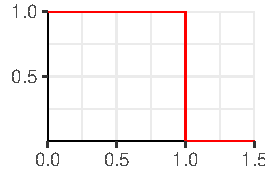
\includegraphics[scale=.66]{./img_ventanas/ventana_bartlett.pdf}
%\\
%\rowcolor{gris}
%Fejer &
%$\displaystyle 
%1-\abso{u}
%$
%& 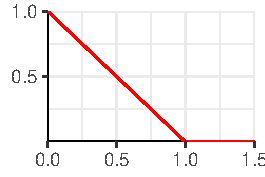
\includegraphics[scale=.66]{./img_ventanas/ventana_fejer.pdf}
%\\
%Daniell &
%$\displaystyle 
%\frac{\SEN{\pi u}}{\pi u}
%$
%& 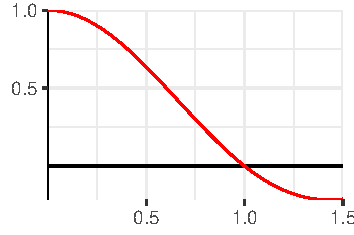
\includegraphics[scale=.66]{./img_ventanas/ventana_daniell.pdf}
%\\
%\rowcolor{gris}
%Parzen (1) &
%$\displaystyle 
%1-u^{2}
%$
%& 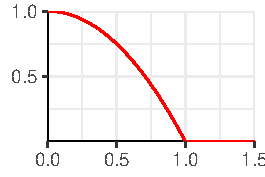
\includegraphics[scale=.66]{./img_ventanas/ventana_parzen1.pdf}
%\\
%Parzen (2) &
%$\displaystyle 
%\frac{1}{1+\abso{u}}
%$
%& 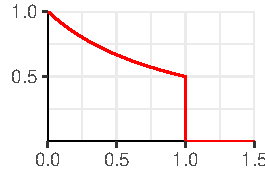
\includegraphics[scale=.66]{./img_ventanas/ventana_parzen2.pdf}
%\\
%\rowcolor{gris}
%Parzen (3) &
%$\displaystyle 
%\frac{1}{1+u^{2}}
%$
%& 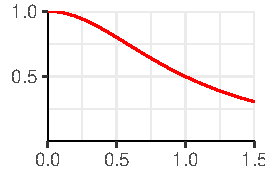
\includegraphics[scale=.66]{./img_ventanas/ventana_parzen3.pdf}
%\\
%Parzen (4) &
%$\displaystyle 
%\begin{cases}
%1-6 u^{2} + 6 \abso{u}^{3} &, \text{ si} \abso{u}\leq \nicefrac{1}{2}\\
%2\left( 1-\abso{u} \right)^{3} &, \text{ otro caso}
%\end{cases}
%$
%& 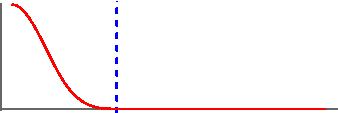
\includegraphics[scale=.66]{./img_ventanas/ventana_parzen4.pdf}
%\\
%\rowcolor{gris}
%Tukey &
%$\displaystyle 
%1 -2a +2a \COS{\pi u}
%$
%& 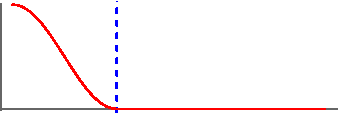
\includegraphics[scale=.66]{./img_ventanas/ventana_tukey.pdf}
%\\
%\bottomrulec
%\end{tabular}
%}
%\caption{Ejemplos de algunas ventanas que suavizan el periodograma}
%\label{ventanas}
%\end{SidewaysTable}

%%%%%%%%%%%%%%%%%%%%%%%%%%%%%%%%%%%%%%%%%%%%%%%%%%%%%%%%%%%%%%%%%%%%%%%%%%%%%%%%%%%%%%%%%%%%%%%%%%%

%\begin{SidewaysTable}
%\centering
%\bordes{1.5}
%\begin{tabular}{c}
%\textbf{Ventanas de retraso tipo escalamiento (2)}
%\vspace{1em}
%\end{tabular}
%
%{
%\begin{tabular}{lll}
%\toprule
%& $k(u)$ para $\abso{u} \leq 1$  & \\
%\midrule
%Neave &
%$\displaystyle 
%\begin{cases}
%1 &, \abso{u}\leq a \\
%\frac{1}{1-a}\left[ 1-u +\frac{b-a}{\pi}\SEN{\frac{b-u}{b-a}\pi} \right] &, a \leq \abso{u}\leq a \\
%\frac{1}{1-a}\left[ 1-u -\frac{1-b}{\pi}\SEN{\frac{u-b}{1-b}\pi} \right] &, b \leq \abso{u} \\
%\end{cases}
%$
%& 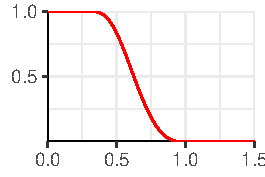
\includegraphics[scale=.66]{./img_ventanas/ventana_neave.pdf}
%\\
%\rowcolor{gris}
%Cuadrática &
%$\displaystyle 
%\frac{25}{12(\pi u)^{2}} 
%\left[ \frac{\SEN{\nicefrac{6 \pi u}{5}}}{\nicefrac{6\pi u}{5}} - \COS{\nicefrac{6 \pi u}{5}} \right]
%$
%& 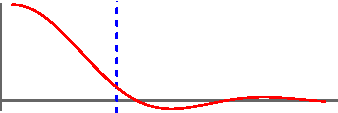
\includegraphics[scale=.66]{./img_ventanas/ventana_cuadratica.pdf}
%\\
%Bartlett-Priestley &
%$\displaystyle 
%\frac{3}{(\pi u)^{2}} \left[ \frac{\SEN{\pi u}}{\pi u} - \COS{\pi u} \right]
%$
%& 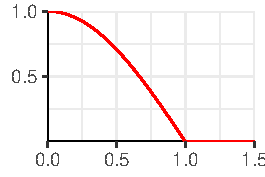
\includegraphics[scale=.66]{./img_ventanas/ventana_cosenoidal.pdf}
%\\
%\rowcolor{gris}
%Papoulis &
%$\displaystyle 
%(1-u)\COS{\pi u} + \frac{\SEN{\pi u }}{\pi u }
%$
%& 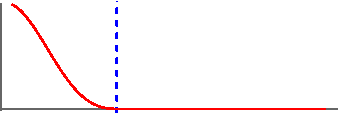
\includegraphics[scale=.66]{./img_ventanas/ventana_papoulis.pdf}
%\\
%Cosenoidal &
%$\displaystyle 
%\COS{\pi u}
%$
%\\
%\rowcolor{gris}
%Trapezoidal &
%$\displaystyle 
%\begin{cases}
%1 &, \abso{u}\leq a \\
%\frac{u-1}{a-1} &, a \leq \abso{u}\leq a 
%\end{cases}
%$
%& 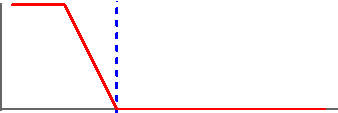
\includegraphics[scale=.66]{./img_ventanas/ventana_trapezoidal.pdf}
%\\
%Normal &
%$\displaystyle 
%\exp \left( - \nicefrac{u^{2}}{2 \sigma^{2}}  \right)
%$
%%& 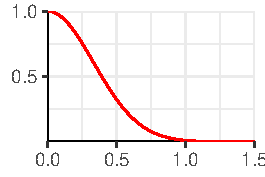
\includegraphics[scale=.66]{./img_ventanas/ventana_normal.pdf}
%& 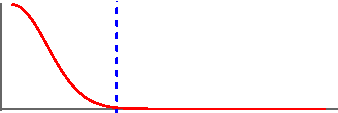
\includegraphics[scale=.66]{./img_ventanas/ventana_.pdf}
%\\
%\bottomrule
%\end{tabular}
%}
%\caption{Ejemplos de algunas ventanas que suavizan el periodograma}
%\end{SidewaysTable}

%%%%%%%%%%%%%%%%%%%%%%%%%%%%%%%%%%%%%%%%%%%%%%%%%%%%%%%%%%%%%%%%%%%%%%%%%%%%%%%%%%%%%%%%%%%%%%%%%%%
%%%%%%%%%%%%%%%%%%%%%%%%%%%%%%%%%%%%%%%%%%%%%%%%%%%%%%%%%%%%%%%%%%%%%%%%%%%%%%%%%%%%%%%%%%%%%%%%%%%
%%%%%%%%%%%%%%%%%%%%%%%%%%%%%%%%%%%%%%%%%%%%%%%%%%%%%%%%%%%%%%%%%%%%%%%%%%%%%%%%%%%%%%%%%%%%%%%%%%%

%\begin{SidewaysTable}
%\centering
%\bordes{1.5}
%\begin{tabular}{c}
%\textbf{Ventanas espectrales tipo escalamiento (1)}
%\vspace{1em}
%\end{tabular}
%
%{
%\begin{tabular}{ll}
%\toprule
%& $K(\theta)$ para $\abso{\theta} \leq 1$ \\
%\midrule
%Bartlett &
%$\displaystyle 
%\frac{1}{\pi} \frac{\SEN{\theta}}{\theta}
%$
%\\
%\rowcolor{gris}
%Fejer &
%$\displaystyle 
%\frac{1}{2\pi} \left[ \frac{\SEN{\nicefrac{\theta}{2}}}{\nicefrac{\theta}{2}} \right]^{2}
%$
%\\
%Daniell &
%$
%\displaystyle 
%\nicefrac{1}{2\pi} \text{, si } \abso{\theta}\leq \pi
%$
%\\
%\rowcolor{gris}
%Parzen (1) &
%$\displaystyle 
%d
%$
%\\
%Parzen (2) &
%$\displaystyle 
%d
%$
%\\
%\rowcolor{gris}
%Parzen (3) &
%$\displaystyle 
%d
%$
%\\
%Parzen (4) &
%$\displaystyle 
%\frac{3}{8 \pi} \left[ \frac{\SEN{\nicefrac{\theta}{4}}}{\nicefrac{\theta}{4}} \right]
%$
%\\
%\rowcolor{gris}
%Tukey &
%$\displaystyle 
%d
%$
%\\
%\bottomrulec
%\end{tabular}
%}
%\caption{Ejemplos de algunas ventanas que suavizan el periodograma}
%\end{SidewaysTable}

%%%%%%%%%%%%%%%%%%%%%%%%%%%%%%%%%%%%%%%%%%%%%%%%%%%%%%%%%%%%%%%%%%%%%%%%%%%%%%%%%%%%%%%%%%%%%%%%%%%

%\begin{SidewaysTable}
%\centering
%\bordes{1.5}
%\begin{tabular}{c}
%\textbf{Ventanas de retraso tipo escalamiento (2)}
%\vspace{1em}
%\end{tabular}
%
%{
%\begin{tabular}{ll}
%\toprule
%& $K(\theta)$ para $\abso{\theta} \leq 1$ \\
%\midrule
%Neave &
%$
%d
%$
%\\
%\rowcolor{gris}
%Cuadrática &
%$\displaystyle 
%d
%$
%\\
%Bartlett-Priestley &
%$\displaystyle 
%\frac{3}{4 \pi} \left[ 1 - \left( \nicefrac{\theta}{\pi} \right) \right]
%\text{, si } \abso{\theta}\leq \pi
%$
%\\
%\rowcolor{gris}
%Papoulis &
%$\displaystyle 
%d
%$
%\\
%Coseno &
%$\displaystyle 
%d
%$
%\\
%\rowcolor{gris}
%Trapezoidal &
%$\displaystyle 
%d
%$
%\\
%Normal &
%$\displaystyle 
%d
%$
%\\
%\bottomrule
%\end{tabular}
%}
%\caption{Ejemplos de algunas ventanas que suavizan el periodograma}
%%\label{ventanas}
%\end{SidewaysTable}

%%%%%%%%%%%%%%%%%%%%%%%%%%%%%%%%%%%%%%%%%%%%%%%%%%%%%%%%%%%%%%%%%%%%%%%%%%%%%%%%%%%%%%%%%%%%%%%%%%%
%%%%%%%%%%%%%%%%%%%%%%%%%%%%%%%%%%%%%%%%%%%%%%%%%%%%%%%%%%%%%%%%%%%%%%%%%%%%%%%%%%%%%%%%%%%%%%%%%%%
%%%%%%%%%%%%%%%%%%%%%%%%%%%%%%%%%%%%%%%%%%%%%%%%%%%%%%%%%%%%%%%%%%%%%%%%%%%%%%%%%%%%%%%%%%%%%%%%%%%
%%%%%%%%%%%%%%%%%%%%%%%%%%%%%%%%%%%%%%%%%%%%%%%%%%%%%%%%%%%%%%%%%%%%%%%%%%%%%%%%%%%%%%%%%%%%%%%%%%%